\section{Prototypes}\todo{More discussion of concepts needed. Design decisions}
This section shows the prototypes that we have made and touches lightly on the application's functionality. The section includes both early and late prototypes to show how the design has progressed and changed. \todo{Billede af start screen}

\begin{figure}[H]
\begin{minipage}[b]{0.5\columnwidth}
\centering
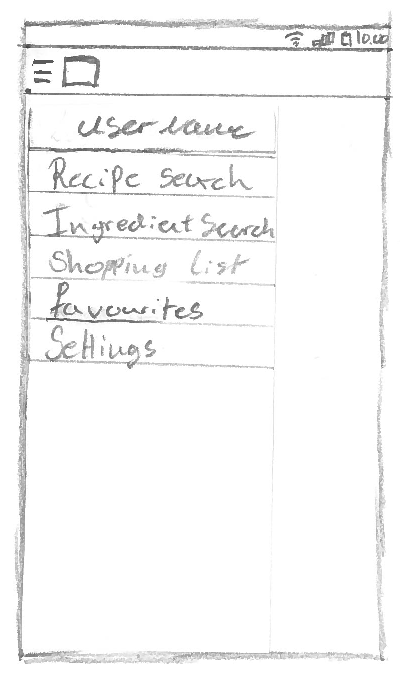
\includegraphics[width=0.7\columnwidth]{img/prototypes/navigation_drawer.pdf}
\caption{The navigation drawer\label{fig:navdrawer}}
\end{minipage}
\hspace{0.5cm}
\begin{minipage}[b]{0.5\columnwidth}
\centering
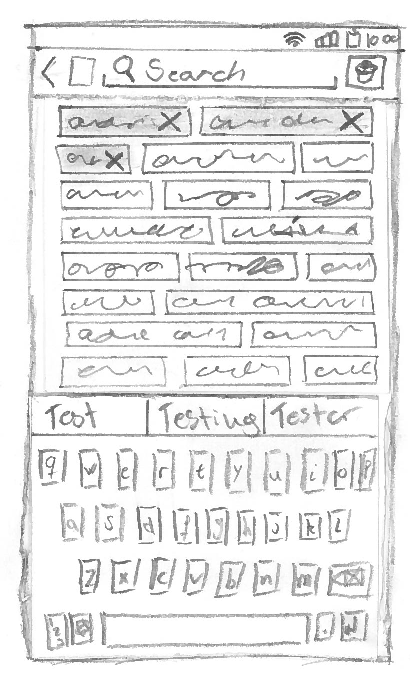
\includegraphics[width=0.7\columnwidth]{img/prototypes/ingredient_search_text.pdf}
\caption{Ingredient search with text\label{fig:ingretext}}
\end{minipage}
\end{figure}

The first thing the user is shown when opening the application is the navigation drawer, as seen on \autoref{fig:navdrawer}. This is a standard component in Android which is used to navigate between different pages\cite{guidelines-navigationdrawer}. We felt that it was a good way to make the views less cluttered, collecting all navigation options in an easy accessible component.

The application allows the user to search for recipes both based on the title of the recipe and based on ingredients that the user inputs. Searching for recipes based on the title is simple and straight forward, the user inputs a partial or full title of the recipe they want and the application shows suggestions based on this. Searching based on ingredients is more complicated. The user might have to type in multiple ingredients and we want to make it easy for them to do so, therefore we have implemented two different ways of aiding the user in entering ingredients, either by text or by tiles.

\autoref{fig:ingretext} shows the screen layout when entering ingredients with text. The user clicks the search field at the top of the page and a keyboard and a word cloud pops up. Now the user can either type in the ingredient they want by use of the keyboard, or if the word appears in the word cloud they can simply click it. The idea with the word cloud is that it comes up with suggestions based on the ingredients the user has already put in.

\begin{figure}[H]
\begin{minipage}[b]{0.5\columnwidth}
\centering
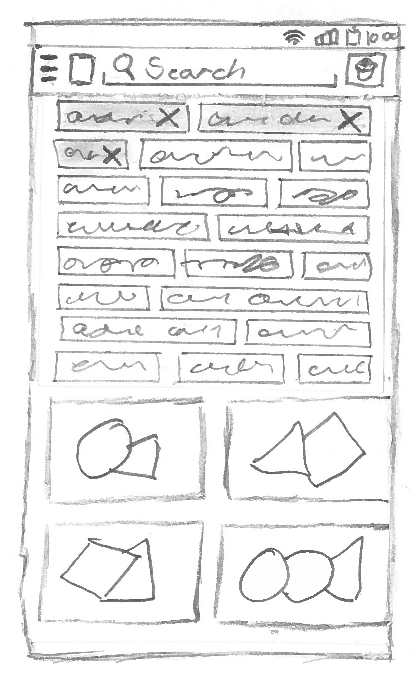
\includegraphics[width=0.7\columnwidth]{img/prototypes/ingredient_search_tile.pdf}
\caption{Ingredient search with tile selection\label{fig:ingreani}}
\end{minipage}
\hspace{0.5cm}
\begin{minipage}[b]{0.5\columnwidth}
\centering
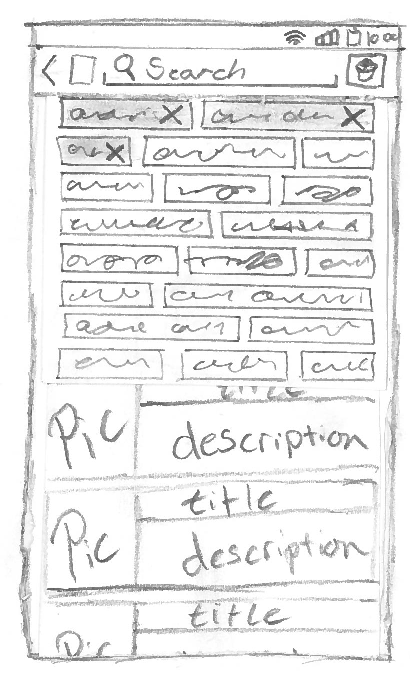
\includegraphics[width=0.72\columnwidth]{img/prototypes/recipe_browse.pdf}
\caption{Recipe browsing with a word cloud\label{fig:recipecloud}}
\end{minipage}
\end{figure}

The same idea applies when entering ingredients using tiles, but instead of a keyboard a small tile bar pops up. This bar contains the different categories, and the user can click on one of these in order to go deeper down into a category, as the user navigates deeper the word cloud will update with words associated with the category they are browsing. The tile navigation can be seen on \autoref{fig:ingreani}. When the user is done with inputting their ingredients they press the back button to close the keyboard or the tiles and can browse the suggested recipes. \autoref{fig:recipecloud}, \autoref{fig:recipestatic}, and \autoref{fig:recipenothing} are three different versions of what it will look like when the user does so.

\autoref{fig:recipecloud} shows the same page without the keyboard, giving the user access to browse the suggested recipes while still having access to the word cloud allowing them to remove or add new ingredients on the fly, however the drawback is a very small view of the suggested recipes. 

\begin{figure}[H]
\begin{minipage}[b]{0.5\columnwidth}
\centering
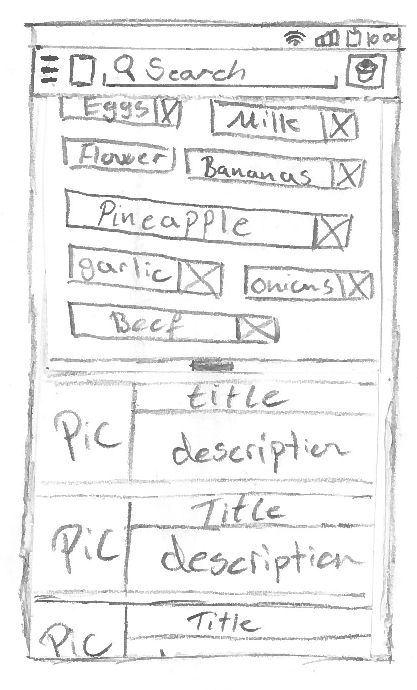
\includegraphics[width=0.7\columnwidth]{img/prototypes/recipe_browse2.pdf}
\caption{Recipe browse with static ingredients\label{fig:recipestatic}}
\end{minipage}
\hspace{0.5cm}
\begin{minipage}[b]{0.5\columnwidth}
\centering
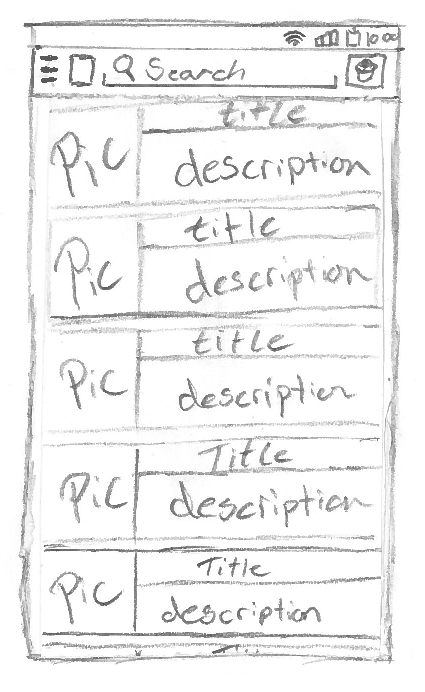
\includegraphics[width=0.7\columnwidth]{img/prototypes/recipe_browse3.pdf}
\caption{Recipe browse without ingredients\label{fig:recipenothing}}
\end{minipage}
\end{figure}

\autoref{fig:recipestatic} shows the page without the keyboard or word cloud but only the selected ingredients, allowing the user to remove items on the fly, again the drawback is a rather small view for the suggested recipes.

\autoref{fig:recipenothing} only shows the suggested recipes, allowing the user to see more recipes but having to click the search field again in order to edit their ingredients.

\begin{figure}[H]
\begin{minipage}[t]{0.5\columnwidth}
\centering
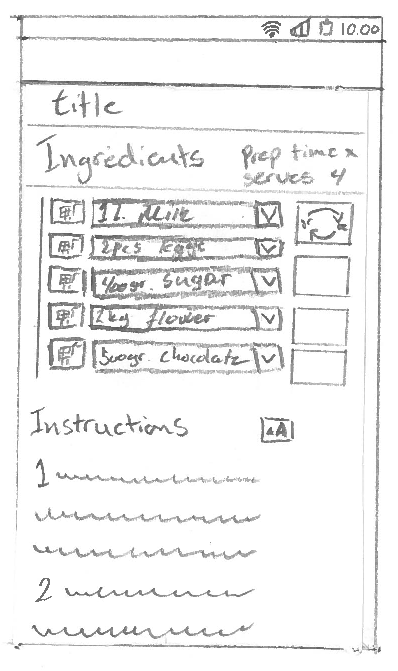
\includegraphics[width=0.7\columnwidth]{img/prototypes/recipe_old.pdf}
\caption{First layout for the recipe view\label{fig:recipeold}}
\end{minipage}
\hspace{0.5cm}
\begin{minipage}[t]{0.5\columnwidth}
\centering
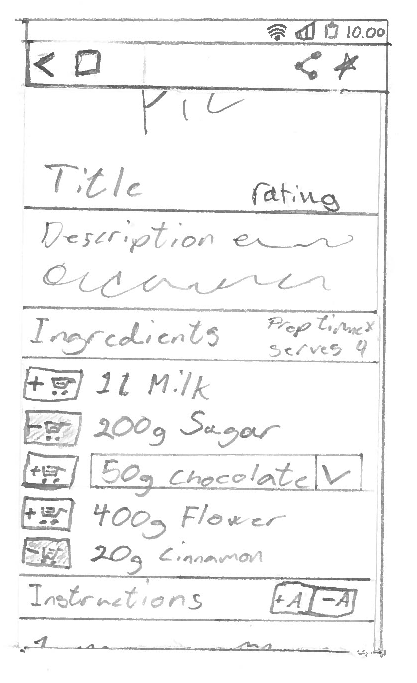
\includegraphics[width=0.735\columnwidth]{img/prototypes/recipe_new.pdf}
\caption{Redesigned recipe layout\label{fig:recipenew}}
\end{minipage}
\end{figure}

When the user finds a suggested recipe they want to look at, they press it and they are taken to a new page. The two variants of this page is shown on \autoref{fig:recipeold} and \autoref{fig:recipenew}. The three vertical lines in the top left corner have been replaced with a back arrow, this indicates two things; the navigation drawer is not available on this page and the back arrow indicates that if you click it you will be taken back to the previous page which is the list of suggested recipes.

In the top right corner there are two new icons; the first button is the share button, allowing the user to share the recipe with their friends and family. The second button is the favourite button, the user can click this to save the recipe under their favourites if they click it again they remove the favourite.

\autoref{fig:recipeold} shows the first design, under the action bar there is a picture of the dish and just under that the title. This is followed by a list of ingredients and the instructions for making the dish. Next to "Ingredients" the user can see the time it takes to prepare the dish, and how many people the dish will serve.

To the left each ingredient there is a button with a shopping cart icon, the user can press this in order to add this ingredient to their shopping list. If the user presses the same icon again, the ingredient is removed from the shopping list. By default the application assumes that the user does not have any of the ingredients, so the user has to choose which ingredients they need to add to the shopping list.

Each of the ingredients have a box around them and a down arrow, this is to indicate a drop down menu. These will appear when an ingredient is exchangeable according to the recipe, meaning the user can use something else similar and still use the recipe. To the right of the ingredients there is a button with a circle on it. If the user presses this button all the unit measures in the recipe will be converted between Imperial and Metric and visa versa. Under the list of ingredients there is a list of instructions telling the user how to cook the dish. The button labelled "aA" next to instructions can be pressed and different font sizes can be chosen.

To the right of the ingredients there is a button with a circle on it. If the user presses this button all the unit measures in the recipe will be converted between Imperial and Metric and visa versa. Under the list of ingredients there is a list of instructions telling the user how to cook the dish. The button labelled "aA" next to instructions can be pressed and different font sizes can be chosen.

We redesigned this layout and the result can be seen on \autoref{fig:recipenew}. Most of the changes are small changes to previous design, for example the location of the title. It has now been moved up onto the picture, together with a rating for the recipe. There is now a small description under the recipe describing the dish. The shopping carts now have a small "+" or a small "-" to indicate if the user will add or delete the ingredient when they press it. We kept the drop down menu for ingredients to indicate that an ingredient is exchangeable. Instead of the "aA" icon that the user should press, there are now two buttons, one to make the font larger and one to make it smaller.

One of the larger redesigns we did, was that we removed the buttons to the right of the ingredients as we decided to add their functionality elsewhere and therefore have more room for the ingredient names.

\begin{figure}[H]
\begin{minipage}[b]{0.5\columnwidth}
\centering
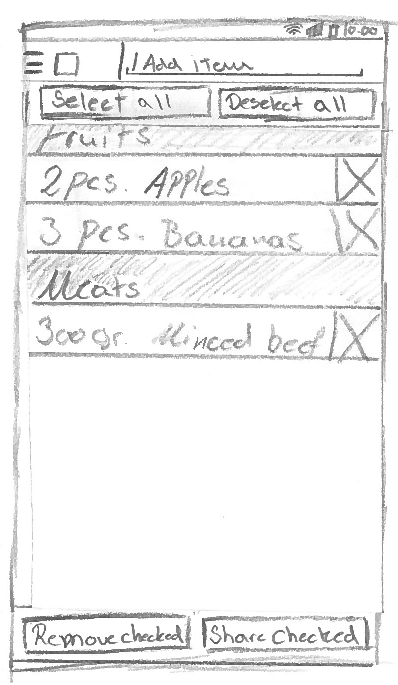
\includegraphics[width=0.7\columnwidth]{img/prototypes/shopping_list_old.pdf}
\caption{First layout for the shopping list\label{fig:shoppingold}}
\end{minipage}
\hspace{0.5cm}
\begin{minipage}[b]{0.5\columnwidth}
\centering
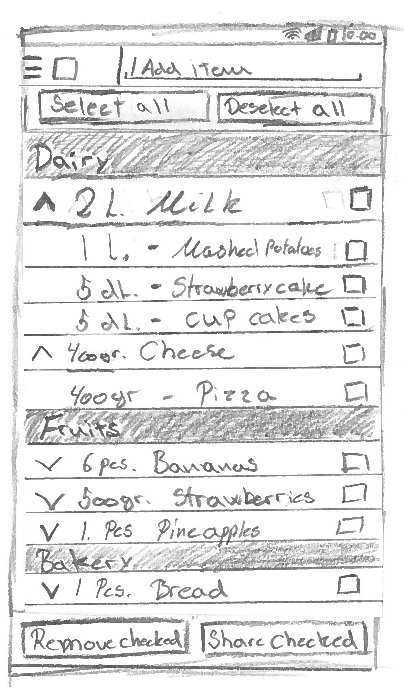
\includegraphics[width=0.7\columnwidth]{img/prototypes/shopping_list_new.pdf}
\caption{Redesigned layout for shopping list\label{fig:shoppingnew}}
\end{minipage}
\end{figure}

The user can always access their shopping list through the navigation drawer. \autoref{fig:shoppingold} and \autoref{fig:shoppingnew} shows the early design and redesign of the shopping list. The user is able to add ingredients directly in the shopping list by clicking the "Add item" field at the top. They are also able to quickly select or deselect all items in the list by clicking the "Select all" or "Deselect all" button under the action bar. This is useful if the user wants to remove all the ingredients or share them all. This can be done through the two buttons at the bottom of the page.

\autoref{fig:shoppingold} shows the first design of the shopping list, it displays how much of each ingredient the user needs, it has a simple layout where ingredients are divided into categories so the user has an easy overview of it. \autoref{fig:shoppingnew} shows a redesigned version of the shopping list. It is designed to show what recipes each ingredient originates from. This means that if the user needs 2L of milk, they can click on it and see in which recipes they need how much milk. It also makes it easier for the user to remove ingredients if they decide not to make a specific recipe.

\begin{figure}[H]
\centering
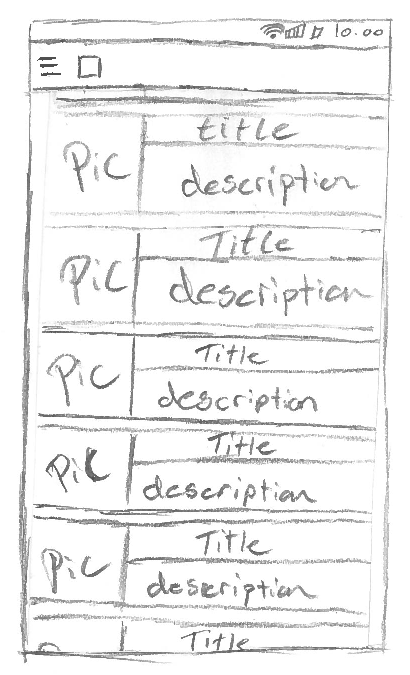
\includegraphics[width=0.35\linewidth]{img/prototypes/favorites.pdf}
\caption{The layout for favourites}
\label{fig:favourite}
\end{figure}

As mentioned before the user can favourite a recipe by clicking the icon when looking at a recipe. \autoref{fig:favourite} shows the favourite page, it looks a lot like \autoref{fig:recipenothing} but it does not have the share or favourite button at the top. The user removes a favourite recipe either by long clicking the recipe or click it to go into the recipe and click the star symbol to remove the favourite.

